\chapter{Laboratorio 2}
\section{Introduzione}
Nell'esperienza di laboratorio precedente, si è realizzato un circuito a guadagno unitario, che realizza una funzione di buffer replicando il segnale in ingresso sull'uscita. Inoltre, esso ha anche una funzione di disaccoppiamento tra ingresso e uscita, con una resistenza di ingresso tendente ad infinito e una resistenza di uscita tendente a zero. 

In questa esperienza di laboratorio, si sono inizialmente effettuate ulteriori misure sul circuito \textit{emitter follower} per poi realizzare una versione \textit{single-ended} dell'\textit{emitter follower}.

\section{Grafico ingresso-uscita \textit{emitter follower}}
Di seguito vengono riportati i risultati delle misure effettuate sul circuito precedentemente realizzato. In ingresso al circuito è stato applicato un segnale sinusoidale con frequenza pari a \SI{1}{\kilo\hertz} e tensione picco-picco variabile da \SI{0.5}{\volt} a \SI{5}{\volt} con step di \SI{0.5}{\volt}. Sono state poi misurate le tensioni picco-picco in ingresso Vpp\sub{i} e in sucita Vpp\sub{o} al circuito grazie alle funzioni integrate dell'oscilloscopio. Per rendere stabile il valore della misura ricavata dall'oscilloscopio, è stato selezionato un filtro a \SI{20}{\mega\hertz} sugli ingressi dell'oscilloscopio e sono state effettuate delle medie (di 6
 campioni) sui segnali. In questo modo è stato possibile ottenere un segnale più pulito da disturbi e rumore (\Fig\ref{fig:emitterfollwer_misurepiccopicco}).
\begin{table}[h!]
	\centering
	\begin{tabular}{c|c}
		\hline
		Vpp\sub{i} [V] & Vpp\sub{o} [V]\\ \hline
		0.509 & 0.491 \\ \hline
		1.019 & 0.984 \\ \hline
		1.502 & 1.476 \\ \hline
		2.080 & 1.994 \\ \hline
		2.565 & 2.474 \\ \hline
		3.037 & 2.962 \\ \hline
		3.524 & 3.459 \\ \hline
		4.022 & 3.967 \\ \hline
		4.606 & 4.470 \\ \hline
		5.089 & 4.945 \\ \hline
	\end{tabular}
\end{table}
\begin{figure}[h!]
	\centering
	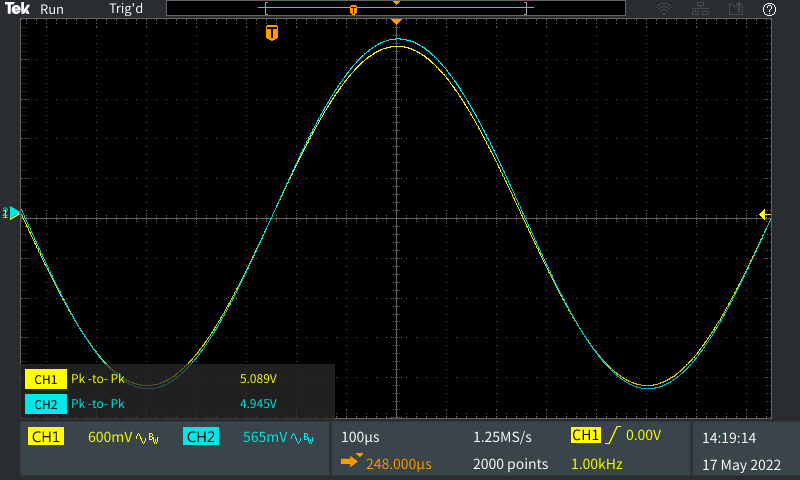
\includegraphics[width=0.7\linewidth]{./ImageFiles/Laboratorio 2/TEK00012}
	\caption{Misurazione della tensione picco-picco del segnale in ingresso (CH1) e in uscita (CH2) con i relativi valori picco-picco misurati dall'oscilloscopio.}
	\label{fig:emitterfollwer_misurepiccopicco}
\end{figure}

\todo{inserire grafico matlab}
